%!TeX root=Main Document/Dissertation.tex
\section{Methodology}
An application was produced to test whether a flock improved by a genetic algorithm can outcompete a flock using a regular expanded boids algorithm in a competitive environment. This application used the Games Education Framework (GEF) [reference] as the framework, which was chosen based on its lightweight overhead, its portability and recommendations from several university lecturers. It was developed using Visual Studio 2017 in C++, chosen due to the ease of working with them and the flexibility afforded by both tools.

GitHub Desktop was used as the tool for source control, ensuring risks to the project were kept to a minimum. Further to this, a GitFlow tool was developed in order to stem the risk of pushing and pulling work from incorrect branches, and prevent any conflicts when committing and pushing new work. The tool essentially acted as a smart checklist; starting a programming session with meant everything was set up correctly before opening individual programs, which happened automatically as the correct items were ticked off.
%%%%%%%%%%%%%%%%


%%%%%%%%%%%%%%%%
\subsection{Test Environment Design}
The application simulated an environment in which two flocks interact (one of which is improved via a genetic algorithm) within a limited space of scarce resources, with the aim of finding out if a flocking algorithm improved by a genetic algorithm can out-compete one without.

To answer the research question required removing as many base assumptions as possible. To do this, three core decisions were made: The environment would be limited so as to keep the flocks in competition with each other, ensuring the flocks would interact; there would be a limited amount of resources in the environment: less than that required to support two full populations of flocks - this would drive the flocks to compete over resources spawned in the environment; finally there would be only two flocks: one improved by a genetic algorithm over simulated generations and one produced through a tested expanded flocking algorithm design. This ensured a competitive environment in which the effects of decisions made by genetic algorithm could be singled out, and the data producing more accurate results. Fig.\ref{fig:EnvScrnshot} displays a screenshot of this environment in action: the red entities representing the regular flock; the blue entities representing the genetic algorithm modified flock; the green entities representing resources in the scene and the white area displaying the space in which the boids can move and interact.
\begin{figure}
	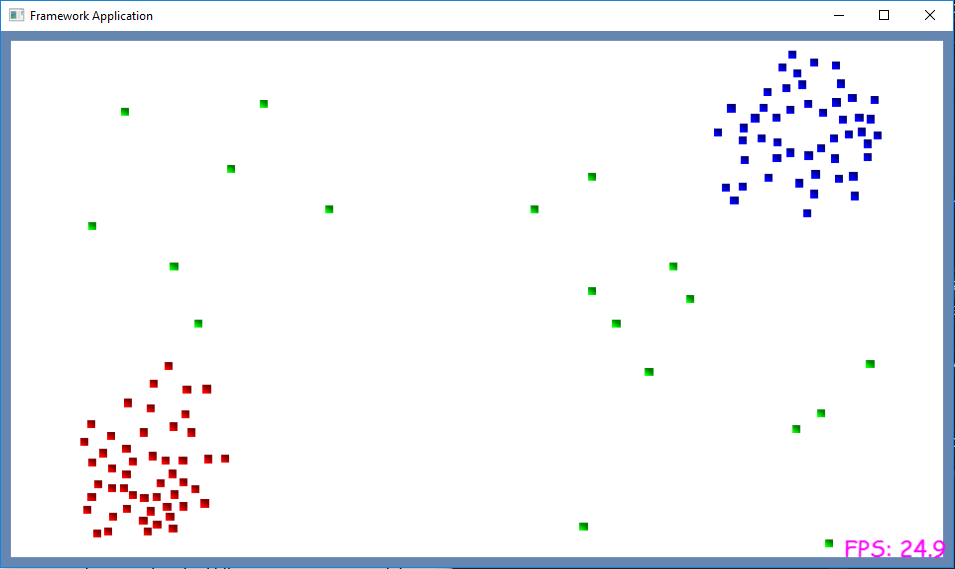
\includegraphics[width=\linewidth]{../Images/EnvironmentScreenshot.png}
	\caption{A screenshot of the test environment in action}
	\label{fig:EnvScrnshot}
\end{figure}
%%%%%%%%%%%%%%%%%%%


%%%%%%%%%%%%%%%%%%%
\subsection{Flocking Algorithm Design}
The original flocking algorithm was designed primarily by adapting the example from \citet{flockingprocessingorg}. This was a very clear representation of how to design a basic flocking algorithm from a code perspective. There were also clear areas for improving the efficiency of the algorithm presented. The most effective way was in combining the calculations for Alignment, Separation and Cohesion. This was to ensure each boid was not checking against all others for each force calculation, and only needed to check against all other boids once instead of three times; doing that was simple and reduced the requirement for N-Body problem solutions like the Barnes-Hut algorithm later on. The other main way was combining the calculations required for each force as they used shared variables, so calculating them once instead of multiple times for each force also increased efficiency.

This worked adequately for the original three forces based on \citet{Reynolds:1987:FHS:37402.37406}. However, issues came up when expanding the application to include extra forces. These were heightened by the fact that, in the aforementioned implementation, it wasn't strictly clear how the forces would graph out due to the lack of separation between direction and weighting. This caused issues to accumulate and it was clear a change in the flocking algorithm design was necessary to expand and edit the program appropriately.

%****[maybe put bit in here about neighbouring boids?? check!! idk if this is the right stage, make sure it makes sense first]****

The boids' forces as they are in the final program were modelled primarily off \citet{4604156}, which has a very clear mathematical representation of each force. The version of the expanded boids algorithm found in this paper was modified by optimising the algorithm for the environment in which it was placed. The forces each boid experienced were: Cohesion, Alignment, Separation, Food Attraction and Flock Avoidance. Each of these forces were the result of multiplication of a unit vector and their respective weight, mathematically represented in Eq.\ref{forcevector_equation}
%****[holy fuck just wanna say this all sounds so smart and just basic grammar/tense changes so far, proud of you]****


\begin{equation}
\boldsymbol{Force Vector} = \boldsymbol{v} \cdot \boldsymbol{w}
\label{forcevector_equation}
\end{equation}
Where $\boldsymbol{v}$ is the unit vector which describes the direction of the force, and $\boldsymbol{w}$ is the weight that magnifies the force dependent on its relation to its environment.

The relationship of the weight to the unit vector will be detailed in relation to boid forces below. Separating direction vector and weight meant it was far easier to mathematically model and graph out each force to predict their behaviour; this reduced in the amount of work necessary to produce a functioning flocking algorithm. The resulting accelerative force then was the sum of these forces. That sum was then used in the Semi-Implicit Euler method to produce the updated position of each boid, every frame.


\subsubsection{Cohesion} 
The first of the boid forces, Cohesion pulls the boid in the direction of flock members, in this case towards its local flock centre. The boids' local flock centre is determined by its neighbours in communicable range and is the average position of those flock members. The further the distance away from its neighbours, the stronger the force. Below is Eq.\ref{cohesion_equation} describing the direction vector and weighting:
\begin{equation}
\begin{split}
	\boldsymbol{\hat{v}_{coh}} &= \frac{ LFCVector} {|LFCVector|} \\
	\boldsymbol{w_{coh}} &= \frac{(|LFCPos - BoidPos|)^2} {30 \cdot FlockSize}
\end{split}
\label{cohesion_equation}
\end{equation}
Where $LFCVector$ represents the vector from the boid to the local flock centre, $LFCPos$ is the position of the local flock centre, $BoidPos$ is the position of the boid and $FlockSize$ is the number of flock members as a whole.

This can be seen visually represented in Fig.\ref{fig:cohesion}. It displays the cohesion force increasing as a boid moved away from the local flock centre.
\begin{figure}
	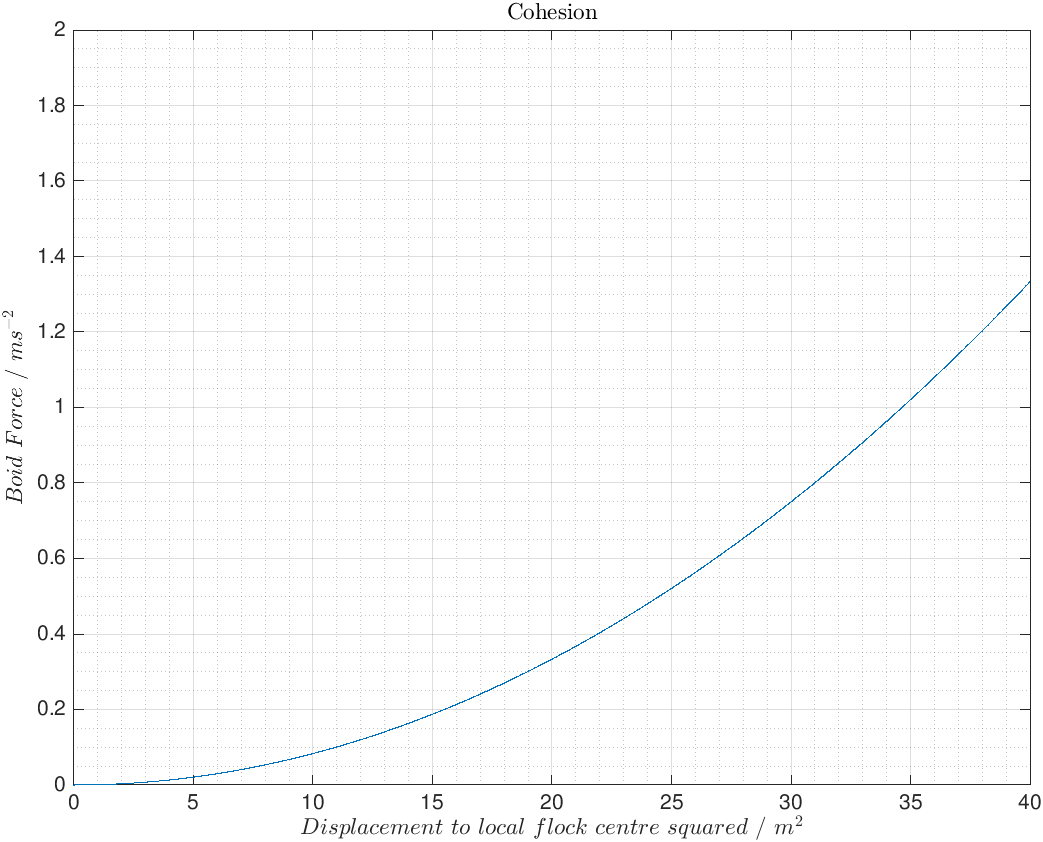
\includegraphics[width=\linewidth]{../Images/cohesion.png}
	\caption{A Graph Displaying the Cohesion Boid Force}
	\label{fig:cohesion}
\end{figure}


\subsubsection{Alignment}
Alignment is a vector which accelerates the boid in the average direction of its neighbouring boids. This produces the common direction of the flock as the boids individually move around. By taking the average velocity of neighbouring boids as a direction vector and multiplying it one over the distance between the local flock centre and the boid itself, a suitable alignment vector is produced. Below is Eq.\ref{alignment_equation} describing the two components of the alignment vector:
\begin{equation}
\begin{split}
	\boldsymbol{\hat{v}_{ali}} &= \frac{ LFVelVector} {|LFVelVector|} \\
	\boldsymbol{w_{ali}} &= \frac{1} {10 \cdot |(LFCPos - BoidPos)|}
\end{split}
\label{alignment_equation}
\end{equation}
Where $LFVelVector$ is the average velocity of the local flock members, and $LFCPos$ and $BoidPos$ are the same as in Eq.\ref{cohesion_equation}.

This can be seen visually represented in Fig.\ref{fig:alignment}. It displays the alignment force increasing as a boid moved closer to the local flock centre.
\begin{figure}
	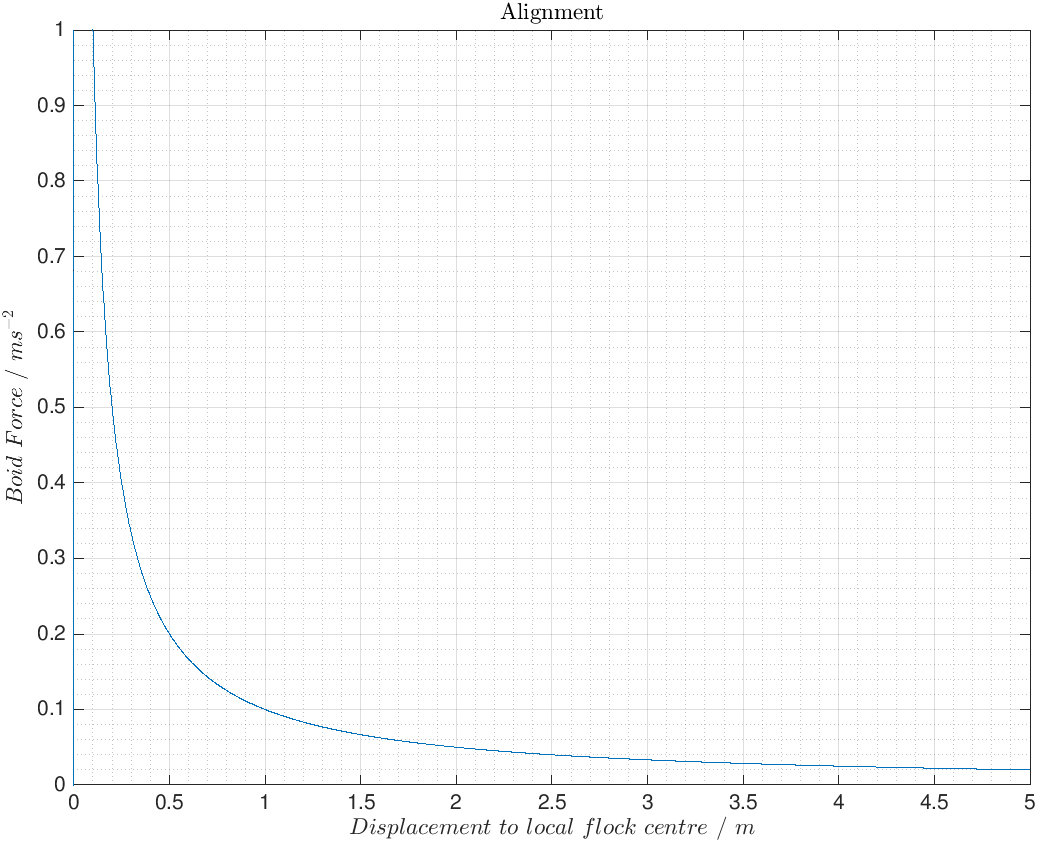
\includegraphics[width=\linewidth]{../Images/alignment.png}
	\caption{A Graph Displaying the Alignment Boid Force}
	\label{fig:alignment}
\end{figure}

\subsubsection{Separation}
Separation is the force that stops the boids from getting too close together. By maintaining enough space between flock members, it grants maneuverability where there would otherwise be collisions (which slow movement down); these could be from obstacles, other moving entities or other boids in the flock. The unit vector that represents the direction for the force to be applied is calculated by taking the negative of the vector to the nearest neighbouring boid; multiplying that by the weighted multiple of the number of neighbours divided by the distance to the closest neighbour produces the separation vector described below in Eq.\ref{separation_equation}:
\begin{equation}
\begin{split}
	\boldsymbol{\hat{v}_{sep}} &= -\frac{ClosestNeighbourVector} {| ClosestNeighbourVector|} \\
	\boldsymbol{w_{sep}} &= 0.025 \cdot  \Big(\frac{NeighbourCount} {|ClosestNeighbourVector|}\Big)^2
\end{split}
\label{separation_equation}
\end{equation}
Where $ClosestNeighbourVector$ is the vector from the boid to the closest neighbour, and $NeighbourCount$ is the number of neighbouring boids.

This can be seen visually represented in Fig.\ref{fig:separation}. It displays the separation force increasing as the displacement between the nearest flock member and itself decreased. This separation force increased for each neighbouring boid.
\begin{figure}
	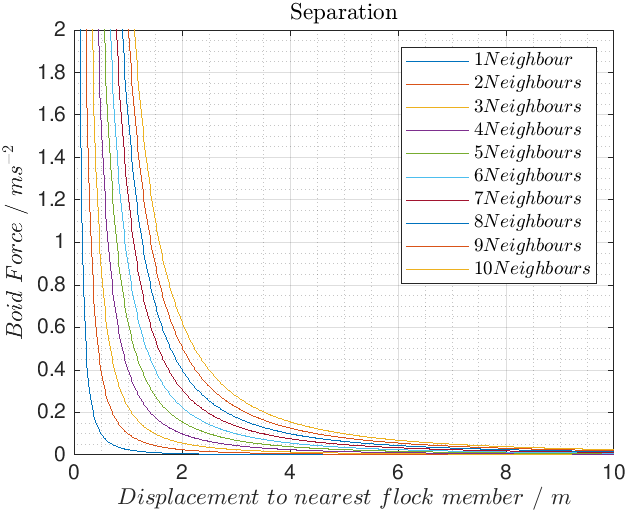
\includegraphics[width=\linewidth]{../Images/separation.png}
	\caption{A Graph Displaying the Separation Boid Force}
	\label{fig:separation}
\end{figure}

\subsubsection{Food Attraction}
This provides an accelerative force toward the nearest resource in the environment. This attraction to nearby food sources is the basis for the boids' survival in the scene. The unit vector to the closest resource gives the direction, and it is the weight which gives its relationship to food in terms of distance away. The equations used are described in Eq.\ref{foodattraction_equation}:
\begin{equation}
\begin{split}
\boldsymbol{\hat{v}_{fda}} &= \frac{ClosestResourceVector} {|ClosestResourceVector|} \\
\boldsymbol{w_{fda}} &= 0.0025 \cdot |ClosestResource|^2 + \frac{36} {|ClosestResource|^2}
\end{split}
\label{foodattraction_equation}
\end{equation}
Where $ClosestResourceVector$ is the vector pointing from the void to the closest resource to it, and $|ClosestResource|$ is the distance to the closest resource.

This can be seen visually represented in Fig.\ref{fig:foodattraction}. It displays relationship the food attraction force has to the displacement squared of the food resource to the boid. It represents two increases in the food attraction force and a minima inbetween, where the food attraction force decreases as the boid gets near to it, but then switches to an increase past a certain point.
\begin{figure}
	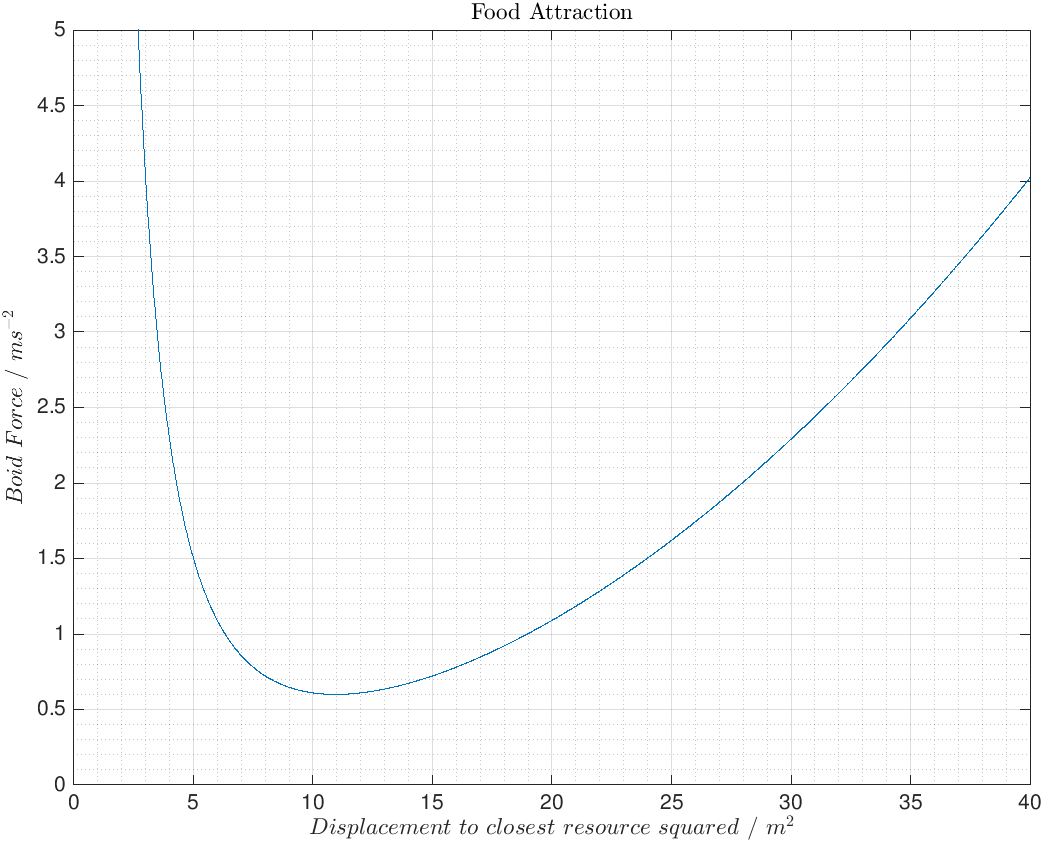
\includegraphics[width=\linewidth]{../Images/foodattraction.png}
	\caption{A Graph Displaying the Food Attraction Boid Force}
	\label{fig:foodattraction}
\end{figure}

\subsubsection{Flock Avoidance}
This is a vector that produces a repelling force away from another flock, and increases as the boid gets closer to the other flock; this is what stops the boids from ignoring each other and keeps them in a competitive environment as they will both be competing for those same resources. The mathematical relationship of the two factors produced can be seen in Eq.\ref{flockavoidance_equation}:
\begin{equation}
\begin{split}
\boldsymbol{\hat{v}_{fla}} &= -\frac{OtherFlockVector} {|OtherFlockVector|} \\
\boldsymbol{w_{fla}} &= \frac{300} {|AvgOtherFlockPos|}
\end{split}
\label{flockavoidance_equation}
\end{equation}
Where $OtherFlockVector$ is the vector pointing from the boid to the average position of another flock within interactable range, and $AvgOtherFlockPos$ is the vector to the average position of another flock within interactable range.

This can be seen visually represented in Fig.\ref{fig:flockavoidance}. It displays the flock avoidance force increasing as a boid moved closer to the local flock centre.
\begin{figure}
	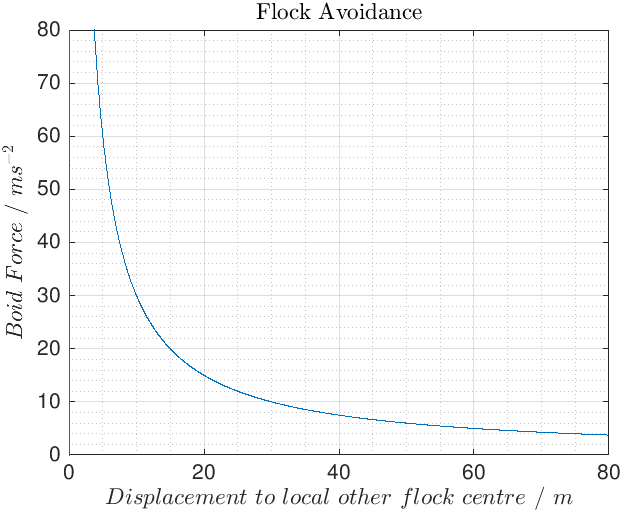
\includegraphics[width=\linewidth]{../Images/flockavoidance.png}
	\caption{A Graph Displaying the Flock Avoidance Boid Force}
	\label{fig:flockavoidance}
\end{figure}
%%%%%%%%%%%%%%%%%%%


%%%%%%%%%%%%%%%%%%%
\subsection{Genetic Algorithm Design}
The functionality for the genetic algorithm (GA) was spread over two classes - genetic\_algorithm and DNA - where the genetic\_algorithm class interacted with the flock and boid classes, and DNA interacted with the genetic\_algorithm and boid classes. The GA had a standard approach to its design which can be seen in Fig.\ref{fig:geneticflow}.
\begin{figure}
	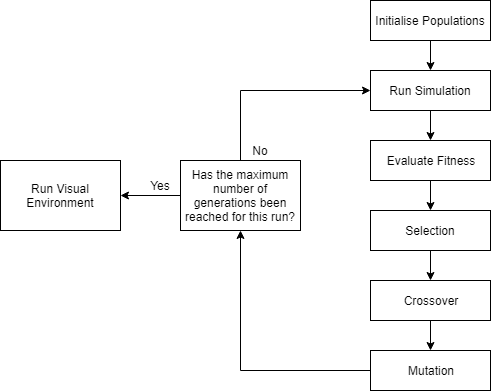
\includegraphics[width=\linewidth]{../Images/GAAlgorithm.png}
	\caption{Flowchart displaying the process the GA takes to improve over time}
	\label{fig:geneticflow}
\end{figure}

Five populations were generated each time the algorithm was initialised; it could be set up to be either random or heuristic, where each population had a random set of data generated for its alleles, and the same but where one population received the heuristic used in the regular flocking algorithm respectively. These populations of boids then made up the genetically enabled flock. 

Each population produced contained chromosomes unique to that population, which is represented by an array in the DNA class. Each GA boid had its own DNA object which is modified by the genetic\_algorithm class. Collectively they made up their respective genotype. Each gene in a chromosome is used in the weight calculations of its respective boid; this can be seen represented below in Eq.\ref{gaweights}:
\begin{equation}
\begin{split}
\boldsymbol{w_{coh}} &= \frac{(chromo[0] \cdot |LFCPos - BoidPos|)^2} {chromo[1] \cdot FlockSize} \\
\boldsymbol{w_{ali}} &= \frac{chromo[2]} {chromo[3] \cdot |(LFCPos - BoidPos)|} \\
\boldsymbol{w_{sep}} &= chromo[4] \cdot \Big(\frac{chromo[5] \cdot NeighbourCount} {chromo[6] \cdot |ClosestNeighbourVector|}\Big)^2 \\
\boldsymbol{w_{fda}} &= chromo[7] \cdot |ClosestResource|^2 + \frac{chromo[8]} {chromo[9] \cdot |ClosestResource|^2} \\
\boldsymbol{w_{fla}} &= \frac{chromo[10]} {chromo[11] \cdot |AvgOtherFlockPos|} 
\end{split}
\label{gaweights}
\end{equation}
Where $chromo[x]$ represents each gene in the chromosome for that boid, changes of the allele of each gene affect the weights in the scene.
These weight calculations made up the phenotype representation in the environment space, and determined the behaviour of a boid. 

\subsubsection{GA Methods}
\paragraph{Evaluation}
At the end of each simulation, each boid was evaluated against the fitness function, which can be seen in Eq.\ref{fitfunc}. The evaluation function then sorted the boids into population types for the selection process. 
\begin{equation}
Fitness Function = BoidHealth + \boldsymbol{w_{1}} \cdot FlockHealth - \boldsymbol{w_{2}} \cdot OtherFlockHealth
\label{fitfunc}
\end{equation}
Where $BoidHealth$ is the health of the boid, $FlockHealth$ is the combined health values of all boids in the flock, and $OtherFlockHealth$ is the combined health of all boids in the competing flock.

This fitness function in Eq.\ref{fitfunc} was designed to take into account the three important factors to a boid in a competitive flock: accounting for its own health was to represent a survival instinct, adding the total flock health to the equation meant improvements to itself over time should be in benefit the flock as a whole, and taking away the weighted total health of the other flock meant the boid had a focus on improving by decreasing the health of the other flock. This fitness function was intended to produce behaviour in the boids that outcompeted the regular flocking algorithm in the environment.

\paragraph{Selection}
The application contained two different kinds of selection algorithm: Roulette Wheel Selection (RWS) and Stochastic Universal Sampling (SUS), both used in answering the research question. In both selection algorithms, increased probabilities of being chosen were given to those populations with better overall fitness. These methods were chosen as they provided selection pressure toward fitter individuals, while also not prematurely coming to a solution which may have been more likely to be a local maxima. 

\paragraph{Crossover}
Crossover of genetic data between parents was done as a single-point crossover that was randomly selected along the genotype, once selected the geneotype halves then got swapped. This was selected due to it being one of the more efficient types of crossover involving the least calculations.

\paragraph{Mutation}
Mutation occured via random increases or decreases of an allele in a randomly selected gene in the genotype, this was intended to be slow enough to not skip over solutions and fast enough to come to solutions quicker.

\subsubsection{Generations}
Part of running the GA was simulating the environment in sped-up runs for the genetic algorithm to improve itself over successive generations. This was done by cutting off unnecessary calculations, that meant all generations occurred in the update function in a loop until the maximum number of generations had been reached. This cut out the requirements for rendering or indeed any calculations not related to the simulation of boid movement and running the genetic algorithm.

The calculations for the simulation physics were also cut down to speed up simulation time in each generational loop. By increasing the time per physics calculation you effectively speed up the time passed each simulation. For example: If one second of simulation time happens in one frame, then if the application runs at sixty frames per second, you can get sixty second of simulation time per real time second, this is displayed in Eq.\ref{speduptime}.
\begin{equation}
	\boldsymbol{SimTime}(s^{-1}) = SimTimeStep \cdot FramesPerSecond
	\label{speduptime}
\end{equation}
Where $SimTime$ is the amount of time passed in simulation per second, $SimTimeStep$ is the difference in time for each calcualtion

Based on this sped up time, each generation had a simulation time limit before moving onto the next one. This had to be balanced as it needed to be a long enough time for real data to come through to get an accurate estimation of fitness and short enough so that the genetic algorithms improvement didn't take too long. The amount of time given per generation will be discussed in the results section as a factor that is controlled for each test due to this.
%%%%%%%%%%%%%%%%%%%%


%%%%%%%%%%%%%%%%%%%%
\subsection{Testing Criteria and Metrics}
The testing criteria has been designed with answering the research question in mind. 

\subsubsection{Controlled Factors}
In a simulations with so many variables, there were many to consider controlling for to identify trends that might otherwise be obscured. In this section will be factors identified as necessary to control for when running the simulation and why. Factors that need to be controlled have been mentioned alongside the results produced where relevant.

Initialising populations was controlled due to two methods being developed in the application, having this controlled meant that it could be made sure there was no effect from changing the population initialisation method. As there were also two different selection menthods developed, controlling for this was important as it was necessary to know in order to make sure runs of the simulation were not accidentally mixed and matched when relevant to producing results, as this could affect the quality of discussion around them and may point toward false conclusions. The selection was always the same during a run of the simulation and so was a factor to consider when producing the data sets. However, this does not need to be controlled for when looking for potential points of convergence in values for each of the boids alleles, as this points toward potential maximas of the solution and is not specific to a selection method.

The probability of mutation was a control factor, keeping it at a fixed value meant the tests could be compared in a temporal manner across generations, especially considering the potential for convergence of data over time. The amount of boids placed in the scene each generation being kept constant meant that the amount of competition for resources was constant across generations and simulation runs. This was similar to the number of resources in the scene, this amount of resources meant more competing with the other flock over food resources, increasing it or decreasing it in different runs could have had an effect on the strategies the flock developed.

\subsubsection{Data Analysis}
\paragraph{Allele}
The frequency of each allele in a gene was used to identify top alleles, and identify if there was convergence of values across simulations. If there was any convergence then that has the potential to be pointing toward maxima in the solution that can point toward the global optimum. 

\paragraph{Genotype}
Analysing the genotype values will give some key results

\paragraph{Phenotype}
How did the genotypical representations identified as important actually have an affect on the boid weights, and so therefore its behaviour in the environment?

\paragraph{GA Flock Strategies}
We will identify observations made about the 

%Maybe write this one once youve actually done the tests youre wanting to talk about tbh because you have zero test design rn, and have given it thought, but not enough to write on, whereas if you just do the tests then you've got a whole thing to setup and the tests can be designed by trial and error. 
%****[AND PLS WRITE IN UR NOTEBOOK AS U GO ALONG - DO A NUMBERED STEP BY STEP FOR URSELF, FEELS TIMECONSUING BUT SOOO FKN TIMEDSAVING IN THE LONG RUN]****

%Test for if the solutions that the GA produce converge at all because thats a sign of potentially finding the global or a significant local maxima in terms of a solution to the problem.
















